\documentclass[10pt,a4paper,twocolumn]{article}
\usepackage[T1]{fontenc}
\usepackage[utf8]{inputenc}
\usepackage{lmodern}
\usepackage[a4paper,margin=20mm,columnsep=7mm]{geometry}
\usepackage{microtype}
\usepackage{amsmath,amssymb}
\usepackage{graphicx}
\usepackage{booktabs}
\usepackage{caption}
\usepackage{listings}
\usepackage{xcolor}
\usepackage[numbers,sort&compress]{natbib}
\usepackage{enumitem}
\usepackage[hidelinks]{hyperref}
\usepackage{url}
\usepackage{tikz}
\usetikzlibrary{arrows.meta,positioning,decorations.pathreplacing}

\captionsetup{font=small,labelfont=bf}
\setlist{nosep,leftmargin=*}
\graphicspath{{../results/}}

\lstdefinelanguage{Faust}{
  morekeywords={process,effect,with,import,library,declare,par,seq,sum,prod,route,ondemand,rdtable,waveform,select2,int,float},
  sensitive=true,
  morecomment=[l]{//},
  morestring=[b]",
}
\lstset{
  language=Faust,
  basicstyle=\ttfamily\scriptsize,
  keywordstyle=\bfseries,
  commentstyle=\color{gray},
  columns=fullflexible,
  keepspaces=true,
  breaklines=true,
  frame=none,
  xleftmargin=0pt,
}

\newcommand{\faustrs}{faust-rs}
\newcommand{\probe}{\texttt{faustprobe}}
\newcommand{\code}[1]{\texttt{#1}}

\title{Same Samples:\\Porting a Block-Based Synthesizer Firmware from C++ to Faust,\\Checked Against the Firmware Itself}
\author{St\'ephane Letz\\GRAME-CNCM, Lyon\\\texttt{letz@grame.fr}}
\date{October 2026}

\begin{document}
\maketitle

\begin{abstract}
Mutable Instruments Elements is a Eurorack modal synthesis voice whose firmware is open source: three exciters (a bow, a blow with a reed tube, a strike that morphs from recorded mallets to bouncing particles), a resonator of 52 zero-delay-feedback band-pass modes with 8 bowed waveguides, a single string or a chord of five dispersive strings, and a reverb whose delay memory is 16 bits, in about 3,700 lines of C++ run at 32\,kHz in blocks of 16 samples. We port all of it to one Faust library, compiled by the Rust Faust compiler \faustrs{}, and ask for the same samples as the firmware, not the same kind of sound. Five things make a block-based engine with a shared random generator into a sample stream that gives its numbers: block-rate work in \code{ondemand} domains clocked by the block start, ramps that accumulate as the C++ accumulates, \code{ondemand} domains that do not fire wherever the C++ skips a computation, so that frozen filters and delay lines resume where they were, delay lines read with the C++'s ring-buffer semantics, and the generator's words handed to each consumer by its $k$-step jump in the C++'s order. Against the firmware's own \code{Part} and \code{Voice}, compiled unchanged, on 11 scenarios that exercise every exciter model, the three resonators, moving parameters, an external input and the reverb, the Faust model agrees to $-72$\,dB of the peak or better in single precision, $-100$\,dB on most; in double precision it drifts where the firmware accumulates phases in float32. A web version plays the model in the browser, lays out 2,000 of its sounds by eight audio measures, and builds phone apps whose controls follow the accelerometer.
\end{abstract}

\section{Introduction}

A port of a synthesizer between languages is usually judged by ear. That judgement is weak where the model is noisy, nonlinear or chaotic: a bowed string, a granular noise or bouncing particles never sound twice the same, and two renders that sound alike can still disagree by several decibels in a register nobody listened to. We take the stance of an earlier port of a physically modelled piano~\cite{coopiano}: the C++ is its own reference. A small program, \code{ref/dump.cpp}, links the firmware's DSP sources~\cite{elements} unchanged, dumps every table the Faust model needs, and renders scenarios through the firmware's \code{elements::Part} (the whole module) and \code{elements::Voice} (the voice alone). The Faust model~\cite{orlarey2009faust} is rendered by \probe{}, the offline probe of \faustrs{}~\cite{faustrs}, under the same control changes at the same samples, and the two are compared sample by sample.

The piano was a model that prepares its notes offline, and its port was a reformulation. Elements is the opposite case: a real-time engine written for a Cortex-M4, whose every sample is already computed in a loop. The difficulty is not to reformulate but to reproduce exactly an engine organized around blocks of 16 samples, with control-rate work at the top of each block, per-block ramps, components that are simply not called when unused, and one random generator shared by four consumers whose draws interleave block by block. Faust has no blocks: a program computes all its signals at every sample. This paper describes how the block structure was written into a sample stream (Sections~\ref{sec:blocks}--\ref{sec:reverb}), what the comparison measures (Section~\ref{sec:results}), and the web version built on the model (Section~\ref{sec:web}).

\section{The firmware}
\label{sec:model}

The DSP of Elements~\cite{elements} (Figure~\ref{fig:arch}) runs at 32\,kHz, the module's codec rate, in blocks of 16 samples (\code{kMaxBlockSize}). \code{Part::Process} reads the patch and the performance state (gate, note, strength, modulation) once per block, renders the voice, mixes it to stereo, soft-limits each channel and applies the reverb.

\begin{figure}[t]
\centering
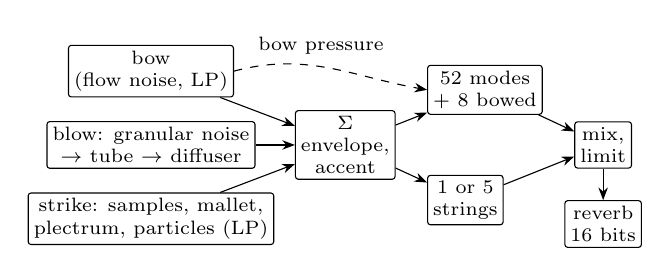
\begin{tikzpicture}[font=\scriptsize, node distance=3mm,
  box/.style={draw, rounded corners=1pt, align=center, inner sep=2pt, minimum height=5mm},
  >={Stealth[length=1.6mm]}]
\node[box] (bow) {bow\\(flow noise, LP)};
\node[box, below=of bow] (blow) {blow: granular noise\\$\to$ tube $\to$ diffuser};
\node[box, below=of blow] (strike) {strike: samples, mallet,\\plectrum, particles (LP)};
\node[box, right=5mm of blow] (sum) {$\Sigma$\\envelope,\\accent};
\node[box, right=4mm of sum, yshift=7mm] (modal) {52 modes\\+ 8 bowed};
\node[box, right=4mm of sum, yshift=-7mm] (str) {1 or 5\\strings};
\node[box, right=4mm of modal, yshift=-7mm] (mix) {mix,\\limit};
\node[box, below=4mm of mix] (rev) {reverb\\16 bits};
\draw[->] (bow) -- (sum);
\draw[->] (blow) -- (sum);
\draw[->] (strike) -- (sum);
\draw[->] (sum) -- (modal);
\draw[->] (sum) -- (str);
\draw[->] (modal) -- (mix);
\draw[->] (str) -- (mix);
\draw[->] (mix) -- (rev);
\draw[->, dashed] (bow.east) to[out=15,in=170] node[above=1pt, pos=0.45]{bow pressure} (modal.west);
\end{tikzpicture}
\caption{The voice and the space section of Elements. The raw excitation, the resonator's center and its side are the voice's three outputs; \code{Part} mixes them by the \emph{space} control.}
\label{fig:arch}
\end{figure}

\paragraph{Exciters.} The \emph{bow} is a value that flips sign when a uniform draw falls under a threshold, mixed with the draw and low-passed by a state-variable filter~\cite{zavalishin2012}; it also sets the bow pressure of the bowed modes. The \emph{blow} reads a 40,963-sample noise recording at a rate set by its timbre and jumps back to a restart point when a draw falls under 1\,\%; above two thirds of its level a reed and bore model in the spirit of McIntyre, Schumacher and Woodhouse~\cite{mcintyre1983} joins in; four all-passes diffuse the result. The \emph{strike} morphs with its meta control between nine mallet and hit recordings (128,013 samples in all, crossfaded two by two), a filtered pulse, a plectrum (a small pulse, then the main one after a delay, and a damping request that mutes the resonator on release) and bouncing particles whose intervals and gains follow random draws. An envelope with four contours (percussive, AD, ADSR, AR) and an accent table driven by the strength input scale them.

\paragraph{Resonator.} The modal resonator~\cite{adrien1991} is 52 band-pass state-variable filters at harmonics of the note stretched by a stiffness that the \emph{geometry} control sets (compressed partials, harmonic, then bars, plates and bells), with Q falling from mode to mode according to \emph{damping} and \emph{brightness}. The modes are summed with the amplitudes of a cosine comb, the frequency-domain image of a pickup at \emph{position}, into the center output, and with those of a second pickup moved by a slow triangle LFO into the side output. The first 8 modes are doubled by bowed waveguides~\cite{essl1999}: a delay line of one period in a loop with a normalized band-pass, all excited by the bow table~\cite{cook1999} of their summed output. Hidden modes replace the resonator by one string or by five strings tuned to a chord: Karplus--Strong strings~\cite{karplus1983,jaffe1983,smith1992} with Hermite-interpolated delay reads, an FIR and an SVF for the damping, dispersion through an all-pass, noise on the delay and a ``curved bridge'' nonlinearity, and a comb pickup; below 15.7\,Hz, where the 2048-sample line is too short, a string runs slower than the sample rate and is upsampled by linear interpolation.

\paragraph{Space.} The \emph{space} control first feeds the raw exciter to the left output, then widens the stereo image, then raises a Griesinger reverberator in the topology described by Dattorro~\cite{dattorro1997}, and freezes it at the end of its travel. Its ten delay lines share one 32,768-cell buffer of 16-bit samples, and two approximate cosine LFOs modulate two of its reads.

\section{From blocks to a stream}
\label{sec:blocks}

\paragraph{The block clock.} The model counts samples from the first one it computes, as the firmware's first block starts at its first sample:
\begin{lstlisting}
bpos = ba.time % BS;          // BS = 16
blk  = bpos == 0;             // the first sample of a block
_hb(x) = (blk, x) : ondemand(_);  // a control held for its block
\end{lstlisting}
In \faustrs{}, \code{ondemand(f)} runs \code{f} only on the samples where its first input is non-zero, holds its outputs otherwise, and advances its state (recursions, delays) once per firing. Everything the C++ computes once per block is such a domain clocked by \code{blk}: the gate flags, the envelope (a five-state machine stepping one phase increment per block), the strike exciter, the chord choice with its hysteresis, the strings' parameters, and \code{Resonator::ComputeFilters}, which refreshes the first 25 modes every block and the 27 others on alternate blocks by the parity of its own call count. The controls are held per block: one moved in the middle of a block acts at the next, as on the module.

\paragraph{Ramps.} The C++ moves a few values across a block by adding, at every sample, an increment computed at the block start, \code{(target - value) / 16}: the envelope, the strength, the pickup position, four string parameters. The sum of 16 increments does not land exactly on the target in float32, and the C++ carries the difference into the next block. \code{\_ramp} does the same, from the value reached at the end of the previous block:
\begin{lstlisting}
_ramp(clk, target, x0) = (\(v, inc).(vn, incn with {
    vp = _init(x0, v);
    incn = _if(clk, (target - vp) / float(BS), inc);
    vn = vp + incn; })) ~ (_, _) : _, !;
\end{lstlisting}

\paragraph{What the C++ does not process.} In string mode the modal resonator is not called; neither are the bowed modes above the number of active modes, the four extra strings in single-string mode, the dispersion all-pass when it is out of the loop, nor a slow string between its ticks. Their filters and delay lines stand still and resume where they were. Each is written as an \code{ondemand} domain whose clock is that condition; a string, for instance, is a domain of the voice, its tick a domain of the string, and the dispersion all-pass a domain of the tick, three levels deep inside recursions. The modes above the number of active ones only keep their state with a select.

\paragraph{Delay lines as ring buffers.} A \code{DelayLine} read at offset $k$ before its write returns what was written $k$ writes ago, and $N$ writes ago when $k$ is a multiple of the size $N$; read after its write, offset $k$ returns what was written $k-1$ writes ago, the current value at 1. The model reads a recursion's fed-back value \code{wp} (what was written one write ago) the same way, \code{\_ring(N, wp, k) = wp @ ((k - 1 + N) \% N)}, which also gives the C++'s corner cases (a comb pickup at less than one sample, a read that wraps).

\section{One shared generator}
\label{sec:random}

\code{stmlib::Random} is one linear congruential generator, $s \mapsto 1664525\,s + 1013904223 \bmod 2^{32}$~\cite{press1992}, shared by the whole voice. Within a block the bow draws once per sample, then the blow once per sample, then the particles of the strike (one word on the gate's rising edge, two or three per bounce, at most one bounce per block since the next interval is at least 96 samples), then each string once per tick (Figure~\ref{fig:words}). The consumers do not draw in time order: the blow's first word of a block follows the bow's last, and the strings' words depend on the particles' bounces in the same block.

\begin{figure}[t]
\centering
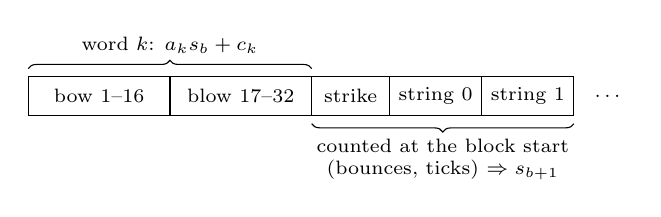
\begin{tikzpicture}[font=\scriptsize, x=0.9mm, y=1mm]
\draw (0,0) rectangle (20,5) node[midway]{bow 1--16};
\draw (20,0) rectangle (40,5) node[midway]{blow 17--32};
\draw (40,0) rectangle (51,5) node[midway]{strike};
\draw (51,0) rectangle (64,5) node[midway]{string 0};
\draw (64,0) rectangle (77,5) node[midway]{string 1};
\node at (82,2.5) {\dots};
\draw[decorate, decoration={brace, amplitude=3pt}] (0,6) -- (40,6) node[midway, above=2pt]{word $k$: $a_k s_b + c_k$};
\draw[decorate, decoration={brace, amplitude=3pt, mirror}] (40,-1) -- (77,-1) node[midway, below=2pt, align=center]{counted at the block start\\(bounces, ticks) $\Rightarrow s_{b+1}$};
\end{tikzpicture}
\caption{The generator's words within one block, in the order the C++ draws them.}
\label{fig:words}
\end{figure}

The model keeps the generator's state $s_b$ at the start of block $b$ and gives every consumer the word it would draw. The state $k$ steps after $s$ is $a_k s + c_k$ with $a_k = a^k$ and $c_k = c\sum_{i<k} a^i$ modulo $2^{32}$, tabulated for $k = 0 \dots 48$ by iterating the C++'s own step; Faust's integers are 32-bit and wrap as the C++'s unsigned arithmetic does. The bow takes word $\code{bpos}+1$ and the blow word $\code{bpos}+17$:
\begin{lstlisting}
bow_sig  = bow_flow(rise & blk, _lcg_jump(bpos + 1, sb), ...);
blow_sig = blow_granular(_lcg_jump(bpos + 17, sb), ...) : tube(...) : ... : diffuser;
\end{lstlisting}
The strike's consumption depends on its own state, so the strike is computed at block rate: \code{random\_block}, clocked by \code{blk}, unrolls the 16 steps of each strike model from word 33 and returns the 16 samples, the damping they request, the strike's state and the generator's state after its draws. Each string then starts after the words of the strings before it; a string below 15.7\,Hz ticks fewer than 16 times per block, so its ticks are counted at the block start by running its resampling phase through the block, the same floating-point operations the string performs sample by sample. The state of the next block follows. Unsigned comparisons flip the sign bit of both operands; unsigned shifts mask; the word becomes a float in $[0,1)$ as \code{GetFloat} makes it.

\section{The reverb in 16 bits}
\label{sec:reverb}

\code{FxEngine} stores each delay line in 16 bits: a write truncates $32768\,x$ to an integer and saturates it, a read divides by 32768. The model quantizes every write the same way (\code{\_q16}) and keeps the unquantized accumulator within the sample, as the C++ does. The first input all-pass is ``smeared'': its line is read at an LFO-modulated offset between 10 and 90 samples, and the interpolated value is written back at offset 100 of the same line, where the all-pass reads its tail 49 samples later. In the model this is a delay of a quantized interpolation:
\begin{lstlisting}
tail1 = _q16(sa + (sb - sa) * o1f) @ 49;   // sa, sb: the line at o1i, o1i + 1
\end{lstlisting}
The two LFOs are approximate cosine oscillators stepped every 32 samples, recursions of coefficient $c = 1.99999702$ for the second one. With $c$ that close to 2, one unit in the last place of a float32 changes the oscillator's frequency by about 2\,\%: the coefficient computed from the C++'s expression in double precision moved the reverb's read offsets enough that the space scenario agreed to $-26$\,dB in single precision; the float32 value, dumped from the C++, brought it to $-74$\,dB. Such constants (two LFO coefficients, the particles' probabilities, the strings' initial delay) are read back from the compiled firmware with the tables.

\section{Results}
\label{sec:results}

\paragraph{Method.} Each scenario is a list of control changes at block boundaries (\code{FRAME NAME VALUE}). The reference program renders it through the firmware's \code{Part} or \code{Voice}, compiled without fused multiply-add so that the compiler cannot change the reference's arithmetic; \probe{} renders the Faust module or voice at 32\,kHz under the same changes, in single and in double precision. The difference is the largest absolute difference over the whole render, in dB of the C++ channel's peak. Table~\ref{tab:results} gives the worst channel of each of the 44 renders (\code{make results}, Apple M5, Apple clang 21, Elements \code{f4cfa76}, \faustrs{} \code{22999fe5}).

\begin{table*}[t]
\centering
\small
\begin{tabular}{llrrrr}
\toprule
 & & \multicolumn{2}{c}{single precision} & \multicolumn{2}{c}{double precision} \\
\cmidrule(lr){3-4}\cmidrule(lr){5-6}
scenario & what it exercises & module & voice & module & voice \\
\midrule
strike & the default patch, a mallet & $-103$ & $-90$ & $-123$ & $-111$ \\
samples & the strike's sample player, three samples & $-98$ & $-82$ & $-52$ & $-35$ \\
plectrum & plectrum and palm mute & $-116$ & $-97$ & $-67$ & $-52$ \\
particles & random bounces, three gates & $-105$ & $-97$ & $-38$ & $-28$ \\
bow & bow, ADSR, moving position and timbre & $-83$ & $-84$ & $-58$ & $-35$ \\
blow & granular noise, then the reed tube & $-105$ & $-95$ & $-56$ & $-46$ \\
string & one string, dispersion, endless damping & $-101$ & $-101$ & $-58$ & $-60$ \\
chords & five strings, a string below 15.7\,Hz, bowing & $-102$ & $-103$ & $-88$ & $-92$ \\
moves & moving parameters, model switched under a note & $-84$ & $-85$ & $-54$ & $-42$ \\
space & raw, stereo, reverb, frozen reverb & $-72$ & $-97$ & $-50$ & $-39$ \\
input & an external signal into the resonator & $-105$ & $-86$ & $-95$ & $-76$ \\
\bottomrule
\end{tabular}
\caption{Largest difference between the Faust model and the firmware over each render (2 to 6\,s), worst channel, in dB of that channel's peak. Module: \code{elements::Part} (main, aux); voice: \code{elements::Voice} (raw, center, side). \code{results/compare.txt} has every channel.}
\label{tab:results}
\end{table*}

\begin{figure}[t]
\centering
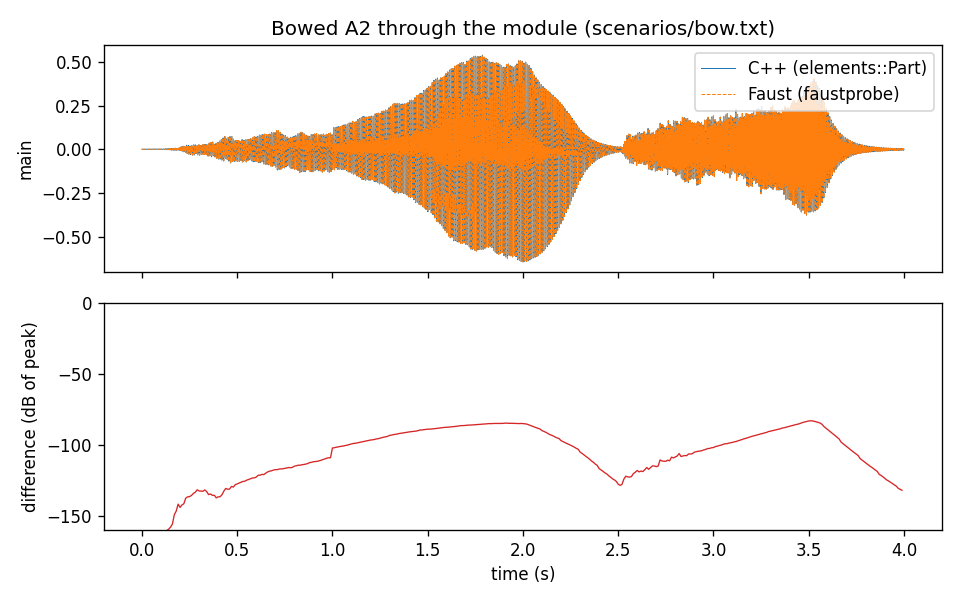
\includegraphics[width=\columnwidth]{fig_bow.png}
\caption{The bow scenario through the module, C++ and Faust superimposed (top) and their difference (bottom), single precision. The bowed modes are a nonlinear loop that amplifies the last-place differences; the worst is $-83$\,dB of the peak.}
\label{fig:bow}
\end{figure}

\paragraph{Single precision.} The model performs the C++'s float operations and should give its float results; it does, to within the reordering of sums and products that the Faust compiler's normal form is free to make, which floating-point arithmetic does not forgive~\cite{goldberg1991}. Where a difference of one unit in the last place crosses a threshold it can grow: the reverb rounds a value to the other 16-bit step and the difference circulates in its loops (space, $-72$\,dB of the peak, $-77$\,dBFS, a few units of the 16-bit memory); the bowed modes amplify it (bow, $-83$\,dB, Figure~\ref{fig:bow}). The random paths, where one flipped comparison would desynchronize a whole note (particles, blow), agree to $-95$\,dB and better.

\paragraph{Double precision.} The firmware accumulates a few phases in float32: the side pickup's LFO phase, the strings' delay ramps, the reverb's LFOs. A double-precision model accumulates the same increments more exactly and drifts away from the firmware (Figure~\ref{fig:precision}). The raw excitation, which accumulates nothing for long, agrees to $-99$\,dB or better in every scenario; the side output and the strings carry the drift.

\begin{figure}[t]
\centering
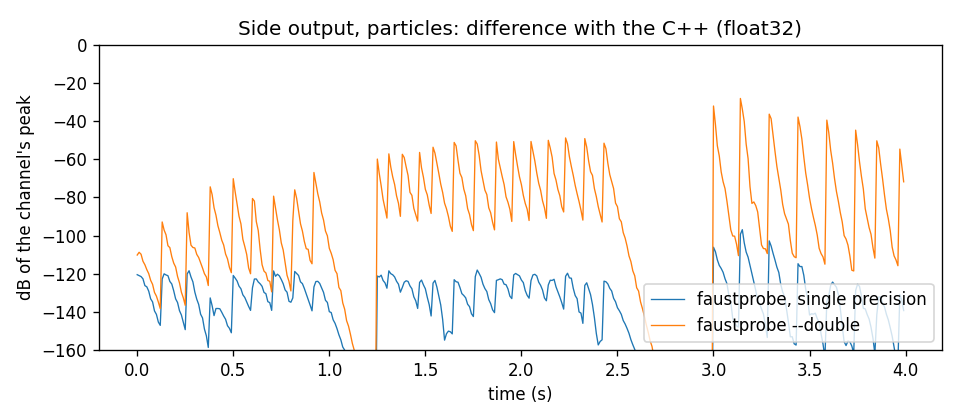
\includegraphics[width=\columnwidth]{fig_precision.png}
\caption{The side output of the particles scenario: difference with the firmware in single and double precision. The double-precision model drifts from the C++'s float32 LFO phase; the single-precision one does not.}
\label{fig:precision}
\end{figure}

\paragraph{Invariances.} The module gives the same samples at host block sizes of 1, 7 and 512 frames, after a reset, and from a second compilation (\probe{} \code{-{}-check all}). The comparison was made to fail once: changing the resonator's input gain from 0.125 to 0.126 gives $-42$\,dB on the center output and a failing exit status.

\paragraph{Cost.} On 100\,s of a held bowed note (\code{make cost}), the firmware's C++ costs 3.5, 1.5 and 4.1\,ms of compute per second of audio with the modal resonator, one string and five strings. The Faust module compiled by \faustrs{} to C++ and by clang at \code{-O3} costs 11.2, 2.9 and 5.1\,ms, and 18.2, 7.4 and 14.3\,ms in \probe{}'s Cranelift JIT. The difference lies in the modes: with 26 modes instead of 52 the native module costs 6.4\,ms instead of 10.4, so the 52 modes are about 8\,ms of its 11.2. The generated code keeps each mode's state in the DSP structure and shifts it every sample where the C++ walks an array of filters; whether that is the whole cause was not measured.

\section{The web version}
\label{sec:web}

The repository's \code{web/} plays the model in a browser, explores its sounds and builds phone apps from them; it is published at \url{https://sletz.github.io/faust-elements/}.

\paragraph{The host.} The voice and the body of the polyphonic program are compiled to WebAssembly by \faustrs{} in single precision and run in an AudioWorklet at 32\,kHz, the browser resampling to the device. A host written for this instrument does what Faust's polyphonic architectures do: the voices' three outputs are summed into one body, and a control goes to every voice and to the body. Every note starts with one 16-sample block with its gate low, so that a key struck again restrikes its own voice on the strings still sounding. A release that arrives before the voice has computed a block with its gate high waits for that block, so that a short click still strikes. A voice that stays below $10^{-5}$ for 1\,s after its release, or for 3\,s while held, stops being computed. Up to 16 voices play, 8 by default. One voice and the body cost 15.6 to 19.3\,ms per second of audio under node, and agree with \probe{} to $-78$\,dB or better.

\paragraph{Divergence.} Elements diverges: a lossless string (damping above 0.95) under a strong bow at a high pitch grows without bound, in the C++ as in the model, to $6\cdot10^{11}$ within 20\,ms. The module resets its voice when the resonator level passes 200; the host clears a voice whose output is not finite or exceeds $10^3$ (the loudest bounded sounds reach about 140), and the body beyond $10^6$. Two thousand random patches through the WebAssembly also found that the side pickup's cosine oscillator diverges when the modulation offset exceeds 0.85 (its amplitudes reach $10^{35}$); the firmware's serial number gives it 0.05 to 0.15, and the control's range now stops at 0.5.

\paragraph{Controls out of range.} Faust does not bound a control by its declared range, and a host may write past it. Each of the 22 controls and the velocity, written well below and above its range through the WebAssembly, should sound exactly as its bound: 27 of the 44 writes did not, seven gave NaN, and five table reads could go past their tables. Every control is now clamped to the range \code{CvScaler} gives it, where it is defined, and the table indices are clamped again as integers inside the functions; all 44 writes sound as their bound, while within the ranges \code{make test} prints the same lines and the atlas below is the same file, byte for byte. A first version also clamped the floating-point argument of the semitone-to-ratio conversion: the compiler then grouped $st + 128$ differently, and single-precision chords moved by one unit in the last place, which the strings amplified.

\paragraph{Exploring the sounds.} Besides one tab per group of controls and 24 presets, two views explore the space of sounds. The orbit of faust-orbit-ui~\cite{faustorbitui} shows every control as a dot to drag, and lays the presets out on a plane by a principal component analysis of their controls, morphing between them by Shepard interpolation. The atlas lays sounds out by what they sound like: 2,000 random patches and the presets, each rendered offline as A3 at velocity 0.7 held 1\,s, are described by eight measures (spectral centroid, spectral flatness, harmonicity, attack, sustain, decay to $-30$\,dB, loudness, stereo width), and placed on the first two principal components of the standardized measures, loudness excepted: the envelope (28\,\% of the variance) and the spectrum (25\,\%). The decay outlasts the render for 65\,\% of the sounds and is extrapolated from the slope of its last 500\,ms. Patches are rendered with their values rounded as stored, since some move by several dB with the fourth digit; eight of them rendered again by \probe{} agree within 0.02\,dB.

\paragraph{The timbre orbit.} A worker measures the current patch after every change, a render and its measures in about 28\,ms, and marks it on the atlas. A second orbit has the eight measures as its dots, each a percentile among the atlas's sounds: moving them asks for a sound, answered by the atlas's nearest sound, then refined by a local search over 40 measured renders. Blending the controls of several neighbours was tried and dropped: over 30 targets, the nearest sound alone is at a median gap of 11 percentiles from the target, a blend of two to six at 21 to 24, since the controls of Elements do not mix linearly into its timbre; the search gains about two points more.

\paragraph{Phone apps.} The page builds a phone app, a progressive web app, from the current sound: a keyboard, an ON/OFF button holding a chosen note as the switch of the SmartFaust apps~\cite{smartfaust}, or both, and controls that follow the axes of the accelerometer with the semantics of Faust's \code{[acc: axis curve amin amid amax]} metadata as faustwasm~\cite{faustwasm} implements them: the axis clipped to its range and mapped by two segments onto the control's minimum, centre and maximum along one of four curves. On a static host the app carries its configuration in its address; its service worker keeps the files for offline use and gives each configuration a manifest of its own, so that several install side by side. A local server can also store built apps and serve them over HTTPS with a local certificate authority, or through a tunnel. The apps were checked in a headless browser (installability, offline playing, motion), not yet on a phone.

\section{What is not ported, and conclusion}

The port needed \code{ondemand} nested three deep inside recursions, 32-bit integer arithmetic that wraps, bit operations for the unsigned comparisons, and \code{waveform} tables of 128,013 samples; all worked as documented, and the voice compiles in 1.2\,s.

The module's easter egg (another synthesis engine), the panic reset of \code{Part} (when the resonator level exceeds 200, which no scenario reaches), and the hardware around \code{Part} (the pots' smoothing and calibration, the input noise gates, the codec's 16-bit conversion) are not ported; the web version clears a diverging voice instead (Section~\ref{sec:web}). In the polyphonic program each voice has its own generator where a \code{Part} with several voices would share one.

A block-based firmware can be written as a Faust stream that gives its samples, not only its sound, if the port is checked against the firmware: the block clock and \code{ondemand} reproduce its control-rate work and its frozen components, the generator's jump reproduces its interleaved random draws, and the float32 constants read back from the compiled C++ reproduce what its arithmetic makes of them. The comparison found what listening would not have: a strike sample player that the port filtered where the firmware does not, 25\,dB too quiet, and a reverb LFO whose frequency depended on one unit in the last place of its coefficient. And the remaining differences have causes: float rounding at the thresholds of a 16-bit memory and of a nonlinear loop, and, in double precision, the firmware's own float32 drift.

\bibliographystyle{plainnat}
\bibliography{references}

\end{document}
